\section{Motivation}\label{sec:motivaiton}
At the beginning, a survey was conducted to check whether more privacy was desired for voice assistants. 110 participants took part in the survey. The participants included the following age groups:
\begin{itemize}
	\item 0 to 18 years 
	\item 19 to 25 years
	\item 26 to 35 years
	\item 36 and older	
\end{itemize}

\begin{figure}[h]
	\centering
	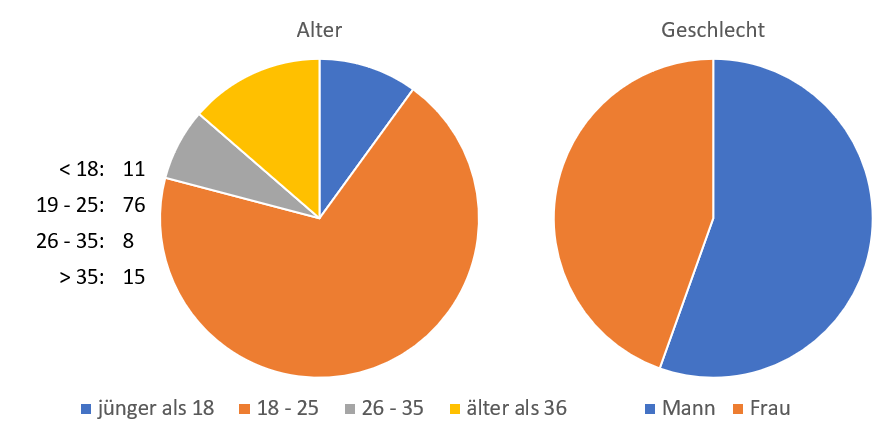
\includegraphics[width=0.9\linewidth]{Picture/umfrage_teilnehmer}
	\caption[Participant of the survey]{Participant of the survey}
	\label{fig:umfrage_teilnehmer}
\end{figure}

55.5\% of the participants were male and 45.5\% female, as shown in Figure \ref{fig:umfrage_teilnehmer}. The participants were asked the following questions:

\begin{enumerate}	
	\item How often do you use a language assistant?
	\item Do you know what happens to your data?
	\item Would you pay money for high data security?
	\item How much money would you pay once for a high data security of an application?
	\item In which applications is privacy especially important to them?
\end{enumerate}

The result of the first question was that 44.5\% of participants use a voice assistant once a month or more frequently. In the US, a study of \glqq highervisibility\grqq{} was conducted, in which more than 70\% of participants use a voice assistant once a month or more \cite{highervisibility}.

A direct comparison of the survey with the study from the USA is shown in Figure \ref{fig: survey_base}. In the study, people in different age groups from different backgrounds were interviewed. The survey conducted under this article was mostly answered by young people.
\begin{figure}[h]
	\centering
	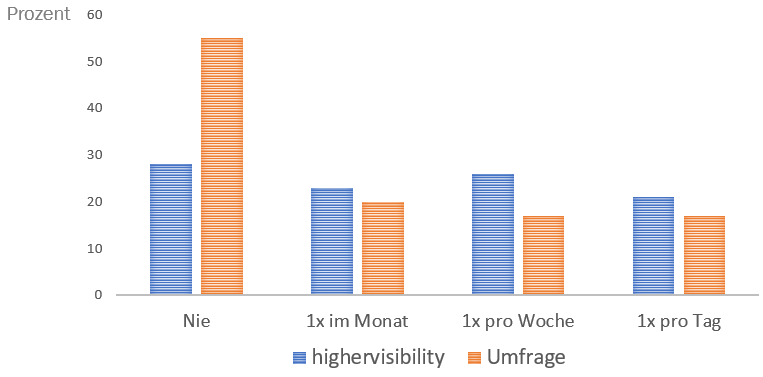
\includegraphics[width=0.9\linewidth]{Picture/umfrage_haeufigkeit}
	\caption[Frequency of use of voice assistants]{Frequency of use of voice assistants}
	\label{fig: survey_base}
\end{figure} 

As can be seen in Figure \ref{fig:umfrage_datenschutz}, 90\% of the participants do not know what's happening to their data. The willingness to pay is visualized by age group in Figure \ref{fig:umfrage_geld_gruppen}. One in four would pay for better data security and 56\% of the participants are unsure whether they would spend money on it. The age rating after willingness to pay is lowest for the group under 18 years of age. The intersection of participants who ticked \glqq Yes\grqq{} or \glqq Maybe\grqq{} increases with age.

\begin{figure}[h]
	\centering
	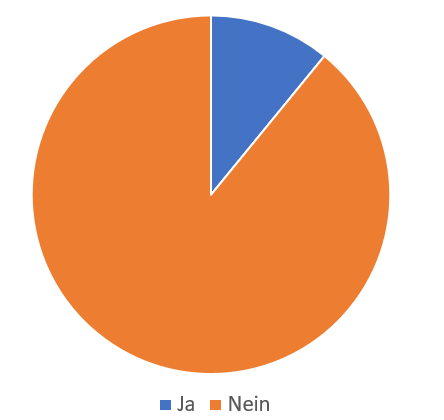
\includegraphics[width=0.5\linewidth]{Picture/umfrage_datenschutz}
	\caption[Relevance of data protection]{Relevance of data protection}
	\label{fig:umfrage_datenschutz}
\end{figure}

\begin{figure}[h]
	\centering
	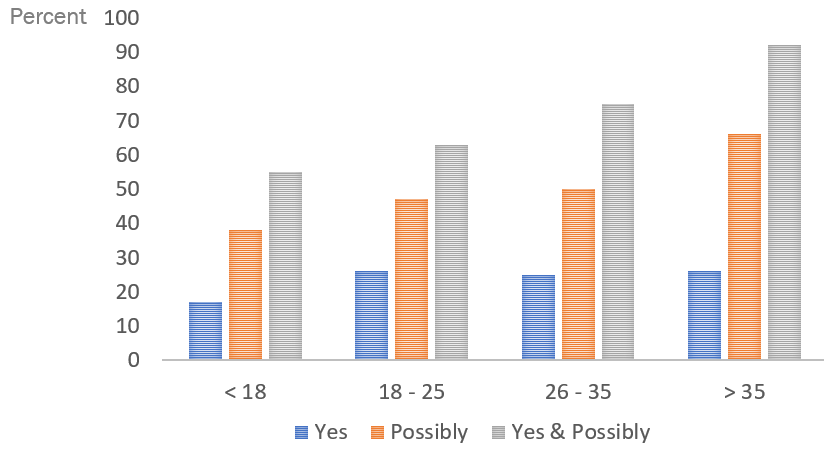
\includegraphics[width=0.9\linewidth]{Picture/umfrage_geld_gruppen}
	\caption[Willingness to pay of different age groups]{Willingness to pay of different age groups}
	\label{fig:umfrage_geld_gruppen}
\end{figure}

The amount that the participants would spend on applications varies a lot and can be seen in Figure \ref{fig:umfrage_betrag}. About 15\% of participants are unwilling to pay, while a majority are ready to pay.

\begin{figure}[h]
	\centering
	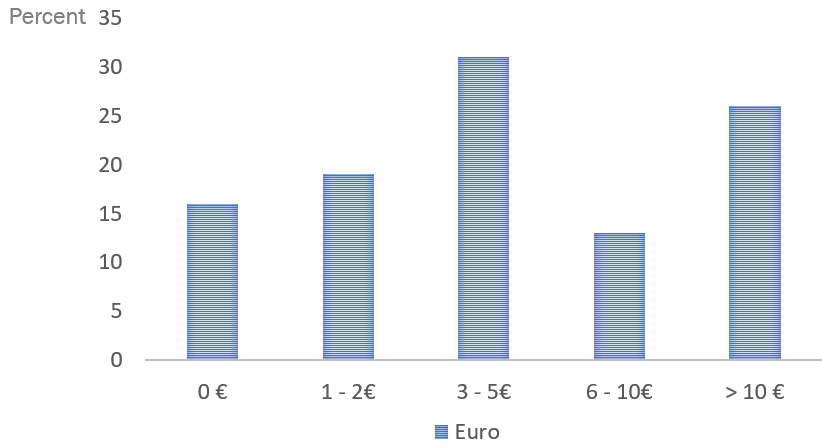
\includegraphics[width=0.9\linewidth]{Picture/umfrage_betrag}
	\caption[Willingness to pay by amount]{Willingness to pay by amount}
	\label{fig:umfrage_betrag}
\end{figure}

As shown in Figure \ref{survey_application}, the privacy of banking, home automation, handset control, social networking and chatting is particularly important to the participants.

\begin{figure}[h]
	\centering
	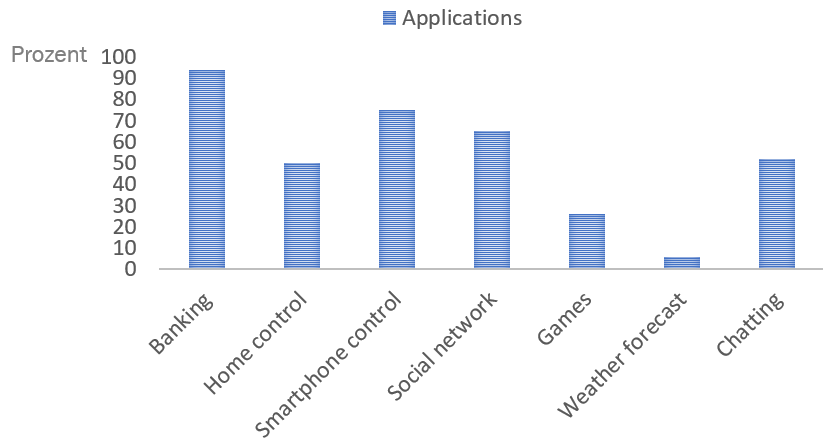
\includegraphics[width=0.9\linewidth]{Picture/umfrage_anwendung}
	\caption[Data protection relevant applications]{Data protection relevant applications}
	\label{survey_application}
\end{figure}

From the surveys, the following conclusions can be drawn:
\begin{itemize}	
	\item Some people use language assistants
	\item Users do not know what's happening to their data
	\item Users would pay for an application if it protects their data
	\item Data protection is important in the areas of banking, chatting, home automation, social media and mobile control.
\end{itemize}
